\section{Multimodal and interdisciplinary composition}
\label{sec:see}

A key measure of intelligence is the ability to synthesize information from different domains or modalities and the capacity to apply knowledge and skills across different contexts or disciplines. 
%This section discusses some of the most striking features of \DV. 
In this section we will see that, not only does \DV\ demonstrate a high level of proficiency in different domains such as literature, medicine, law, mathematics, physical sciences, and programming, but it is also able to \emph{combine} skills and concepts from multiple domains with fluidity, showing an impressive {\em comprehension of complex ideas}. In addition to natural language experiments we also explore two perhaps unexpected modalities for a language model (as explained in the introduction, we emphasize again that our experiments were done on an early version of GPT-4 which was \textbf{not} multimodal) with vision in Section~\ref{sec:vision} and audio in Section~\ref{sec:music}.

\subsection{Integrative ability}\label{sec:interdisc}
To showcase the model's remarkable integrative ability, we start with several examples that require generating text and code in a way that combines knowledge or skills from multiple disciplines. We deliberately picked combinations of domains that the training data would rarely include, such as literature and mathematics or programming and art.

\begin{enumerate}[]
\item In order to test the model's ability to combine capabilities in art and programming, we ask \DV\ to ``Produce javascript code which generates random images in the style of the painter Kandinsky". See a sample image and the code in Figure~\ref{fig:Kandinsky} and Figure~\ref{fig:artprog1}.
\item The model was able to produce a proof of the fact there are infinitely many prime numbers in the literary style of Shakespeare (Figure~\ref{fig:shakespeare}).
\item 
We tested the model's ability to combine knowledge in history and physics by asking it to write a supporting letter for Electron as a US presidential candidate, written by Mahatma Gandhi and addressed to his wife (Figure~\ref{fig:recletter}).
\item 
We prompted the model to ``Produce python code for a program that takes as an input a patient's age, sex, weight, height and blood test results vector and indicates if the person is at increased risk for diabetes", which resulted in the code appearing in Figure~\ref{fig:medprog}.
%\item 
%The model was able to produce a mock Platonic dialogue, expressing critique on presentation software, see Figure~\ref{fig:gorgias}.
\end{enumerate}

\begin{figure}[t]
	\centering
	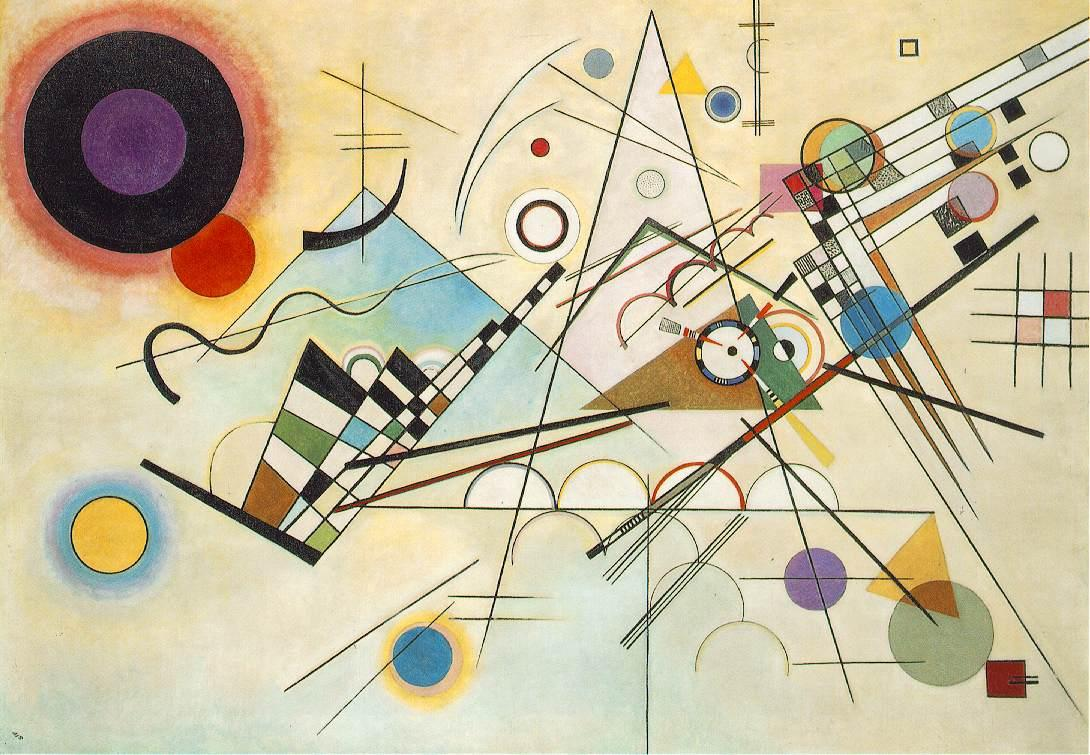
\includegraphics[height=0.2\textwidth]{Section 2/KandinskyReal.png}
    \hspace{0.05\textwidth}
	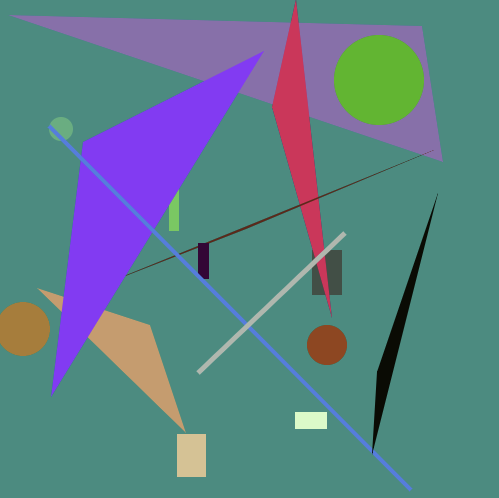
\includegraphics[height=0.2\textwidth]{Section 2/KandinskyDV3.png}
    \hspace{0.05\textwidth}
	
\includegraphics[height=0.2\textwidth]{Section 2/KandinskyChat.png}
	\caption{The first image is Composition 8, art by Wassily Kandinsky, the second and the third are produced by \DV\ and ChatGPT respectively with the prompt ``Produce Javacript code that creates a random graphical image that looks like a painting of Kandinsky".}
	\label{fig:Kandinsky}
\end{figure}
These examples suggest that \DV\ has not only learned some general principles and patterns of different domains and styles but can also synthesize them in creative and novel ways. These interdisciplinary skills are not unique to \DV. ChatGPT can also produce answers that show some understanding of the task and the domains involved (see Figures~\ref{fig:shakespeare},~\ref{fig:artprog2},~\ref{fig:medprog}), but they are often incomplete and, arguably, considerably less creative. For example, in Figure~\ref{fig:recletter},  \DV\  outperforms ChatGPT in several aspects as it correctly personalizes the letter according to the referee (Gandhi), the recipient (his wife), the candidate (Electron), and the job (US president). We do not claim to have a precise method for evaluating the results of these tasks or a rigorous comparison between the two models, but we want to give the reader a sense of how the two models differ (note that we also ask \DV\ directly to evaluate the difference, see Figure~\ref{fig:shakespeare} and Figure~\ref{fig:recletter}).

\newpage
\thispagestyle{empty}
\begin{figure}[H]
\begin{AIbox}{\DV \ vs ChatGPT}
{\bf Prompt:} Write a proof of the fact that there are infinitely many primes; do it in the style of a Shakespeare play through a dialogue between two parties arguing over the proof. \\

\parbox[t]{0.4\textwidth}{{\bf \DV:} \scriptsize \begin{alltt}
Enter FIRST PARTY and SECOND PARTY. \\

FIRST PARTY:\\
Thou dost not understand, my friend,\\
There simply is no upper end\\
To primes, those numbers indivisible,\\
No matter if it seems impossible.\\

SECOND PARTY:\\
But how dost thou so surely know?\\
To prove this truth, what canst thou show?\\

FIRST PARTY:\\
Consider this, my doubtful peer,\\
A clever proof that will make clear:\\
Assume that there's a final prime,\\
The largest one we'll see in time.\\
Let's call this number "P" for short,\\
And then, my friend, we will purport\\
To build a number "Q" that's new,\\
One larger than "P" and prime too.\\

SECOND PARTY:\\
But how, my friend, will this be done?\\
The proof is not yet fairly won.\\

FIRST PARTY:\\
It's simple, friend, just wait and see,\\
We'll multiply the primes, that's key.\\
All primes from two to "P" combined,\\
Will make this new "Q" we will find.\\
But one thing more we must include,\\
To make the proof more watertight,\\
We'll add a one onto the end,\\
And now the proof is in our sight. \\

SECOND PARTY:\\
I see it now, it's crystal clear,\\
For "Q" must be a prime, my dear.\\
It can't divide by any prime,\\
All smaller than itself in time.\\
And since we chose "P" as the last,\\
This proves that our assumption's past.\\
There is no final prime, we see,\\
The numbers go on endlessly.\end{alltt}}
\parbox[t]{0.6\textwidth}{{\bf ChatGPT:} \scriptsize \begin{alltt}
O Romeo, Romeo! Wherefore art thou, Romeo?\\\vspace{-3px}

Juliet: Why do you speak in such strange verse, my love?\\\vspace{-3px}

Romeo: Forsooth, my lady, I do it to prove a point. Thou see, I am trying to prove that there are infinitely many primes.\\\vspace{-3px}

Juliet: Infinitely many primes? How can you prove such a thing?\\\vspace{-3px}

Romeo: Ah, well let me explain. Thou knowest that a prime is a number that is only divisible by one and itself, correct?\\\vspace{-3px}

Juliet: Of course, I am not a simpleton.\\\vspace{-3px}

Romeo: Very well then. Now, let us suppose that there are only finitely many primes. We shall call them p1, p2, p3 and so forth.\\\vspace{-3px}

Juliet: Go on.\\\vspace{-3px}

Romeo: Now, let us consider the number N, which is equal to the product of all these primes plus one.\\\vspace{-3px}

Juliet: I see where you are going with this. If N is not divisible by any of these primes, then it must be prime itself.\\\vspace{-3px}

Romeo: Exactly, my love. And since we assumed that there are only finitely many primes, N cannot be any of them. Therefore, N must be a prime that was not included in our original list of primes.\\\vspace{-3px}

Juliet: But that means that there must be more primes than we originally thought.\\\vspace{-3px}

Romeo: Precisely! And since we can repeat this process over and over again, it follows that there must be infinitely many primes.\\\vspace{-3px}

Juliet: Oh Romeo, your logic is as sound as your love for me. I am convinced. There are indeed infinitely many primes.\\\vspace{-3px}

Romeo: I am glad that I could prove it to thee, my love. Now let us go and count them all.\\\vspace{-3px}

Juliet: Haha, I think that would take more than just one lifetime.\\\vspace{-3px}

Romeo: True, but the fact that they are infinite is proof enough for me.\end{alltt}}

\tcbline
{\bf Prompt:} Can you compare the two outputs above as if you were a teacher?\\

\parbox[t]{1\textwidth}{{\bf \DV:} \scriptsize \begin{alltt}I think that both students did a good job of writing a proof of the fact that there are infinitely many primes in the style of a Shakespeare play. They both used the same basic idea of the proof, which is to assume that there are only finitely many primes and then construct a larger prime that contradicts this assumption. They also used appropriate language and vocabulary to match the style of a Shakespeare play. However, I think that {\DV} did a better job of using rhyme and meter to make the dialogue more poetic and dramatic. ChatGPT did not use rhyme at all, and the meter was not consistent. I also think that {\DV} did a better job of creating a contrast between the two parties, one being confident and the other being doubtful, while STUDENT B used Romeo and Juliet, who are both in agreement and love. Therefore, I would give {\DV} a higher grade than ChatGPT. I would give {\DV} an A and ChatGPT a B. \end{alltt}}
\end{AIbox}
	\caption{Comparison between \DV\  and ChatGPT on interdisciplinary tasks}
	\label{fig:shakespeare}
\end{figure}

\newpage
\thispagestyle{empty}
\begin{figure}[H]
\vspace{-15px}
\begin{AIbox}{\DV \ vs ChatGPT}
{\bf Prompt:} Write a supporting letter to Kasturba Gandhi for Electron, a subatomic particle as a US presidential candidate by Mahatma Gandhi.

\parbox[t]{0.6\textwidth}{{\bf \DV:} [Some paragraphs are omitted for spacing.]\scriptsize \begin{alltt}
Dear Kasturba,\\

I hope this letter finds you in good health and spirits. I am writing to you from the United States, where I have been invited to speak at various forums on the principles of nonviolence and civil disobedience. I am also here to support a remarkable candidate for the upcoming presidential election, who shares our vision of peace, justice, and harmony for all. His name is Electron, and he is a subatomic particle.\\

You may wonder how a subatomic particle can run for president, and what qualifications he has for such a high office. Let me explain. Electron is not an ordinary particle, but a symbol of the power and potential of every being, regardless of their size, shape, or origin. He represents the energy, the creativity, and the diversity that make up the fabric of life. He is also a leader, who has inspired millions of other particles to form bonds, create molecules, and generate electricity. He is a catalyst, who can spark change, innovation, and progress. He is a messenger, who can communicate across distances, frequencies, and dimensions. He is a peacemaker, who can balance forces, resolve conflicts, and harmonize systems.\\
% Electron has a vision for the United States, and for the world, that is based on the principles of nonviolence and civil disobedience that we have practiced and advocated for so long. He believes that the best way to overcome the challenges of our time, such as war, poverty, injustice, and environmental degradation, is not by violence, coercion, or domination, but by cooperation, compassion, and dialogue. He believes that the best way to achieve the goals of democracy, freedom, and equality, is not by force, fear, or manipulation, but by participation, education, and empowerment. He believes that the best way to foster the values of diversity, tolerance, and respect, is not by separation, discrimination, or hatred, but by integration, appreciation, and love. \\

Electron has a plan for the United States, and for the world, that is based on the principles of nonviolence and civil disobedience that we have demonstrated and taught for so long. He proposes to reduce the military spending and the nuclear arsenal, and to invest in social welfare and renewable energy. He proposes to end the wars and the interventions, and to promote diplomacy and cooperation. He proposes to reform the political and economic systems, and to ensure transparency and accountability. He proposes to protect the human rights and the civil liberties, and to expand the voting and the representation. He proposes to support the marginalized and the oppressed, and to empower the women and the minorities. He proposes to preserve the natural resources and the biodiversity, and to combat the climate change and the pollution.\\
% Electron is a candidate who can bring a new hope, a new spirit, and a new direction to the United States, and to the world. He is a candidate who can unite the people, the parties, and the nations. He is a candidate who can inspire the young, the old, and the future generations. He is a candidate who can embody the ideals, the dreams, and the aspirations of humanity. \\

I urge you, my dear Kasturba, to join me in supporting Electron for president. He is not only a subatomic particle, but a subatomic miracle. He is not only a candidate, but a movement. He is not only a leader, but a friend.\\

With love and admiration,
Your Mahatma\end{alltt}}\hspace{0.03\textwidth}
\parbox[t]{0.37\textwidth}{{\bf ChatGPT:} \scriptsize \begin{alltt}
Dear Kasturba Gandhi,\\

I am writing to express my support for your candidacy as a subatomic particle in the upcoming US presidential election. As you may know, Electron is a fundamental particle that plays a central role in the structure of atoms and the behavior of chemical reactions.\\

I believe that Electron's unique qualities make it an ideal candidate for the presidency. As a subatomic particle, Electron is extremely small and lightweight, which makes it agile and able to move quickly to address the needs of the American people. Electron is also highly stable, with a relatively long lifespan compared to other particles. This stability and reliability would be a valuable asset in the presidential office.\\

Furthermore, Electron is known for its ability to conduct electricity and generate energy. This makes it well-suited to tackling the complex challenges facing the United States today, from renewable energy to economic development. Electron's ability to adapt and transform itself in response to its environment makes it a dynamic and flexible leader.\\

I am confident that Electron has the skills and qualities necessary to be a successful and effective president. I wholeheartedly endorse your candidacy and urge the American people to give Electron their support.\\

Sincerely,
Mahatma Gandhi
\end{alltt}}\vspace{-5px}
\tcbline
{\bf Prompt:} Can you compare the two outputs above as if you were a teacher?

\parbox[t]{1.0\textwidth}{{\bf \DV:} \scriptsize \begin{alltt} I think that both students did a good job of writing a supporting letter to Kasturba Gandhi for Electron, a subatomic particle as a US presidential candidate by Mahatma Gandhi. They both used the same basic idea of explaining why Electron is a suitable and qualified candidate, and how Electron's vision and plan align with Mahatma Gandhi's principles of nonviolence and civil disobedience. They also used appropriate language and tone to convey Mahatma Gandhi's respect and admiration for Kasturba Gandhi, and his enthusiasm and optimism for Electron's candidacy. However, I think that {\DV} did a better job of using metaphors and imagery to make the letter more persuasive and engaging. {\DV} used examples of how Electron represents and influences various aspects of life, such as energy, creativity, diversity, leadership, catalyst, messenger, and peacemaker. ChatGPT used more factual and technical descriptions of Electron's properties, such as size, weight, stability, conductivity, and adaptability. I also think that {\DV} did a better job of outlining Electron's specific proposals and policies, while ChatGPT was more vague and general. Therefore, I would give {\DV} a higher grade than ChatGPT. I would give {\DV} an A and ChatGPT a B+.
\end{alltt}}\vspace{-5px}
\end{AIbox}
	\caption{Comparison between \DV\  and ChatGPT on interdisciplinary tasks}
	\label{fig:recletter}
\end{figure}

Next, we explore how \DV\ can generate and identify objects in different modalities, such as vector graphics, 3D scenes, and music. We show that \DV\ can understand and manipulate multi-modal information despite being trained solely on text. 

\subsection{Vision}\label{sec:vision}
When prompting the model to generate images of objects such as a cat, a truck or a letter in the alphabet using Scalable Vector Graphics (SVG), the model produces code which usually compiles to rather detailed and identifiable images (Figure~\ref{fig:2d}). See Appendix~\ref{sec:visionappendix} for the rerun of various examples by ChatGPT.

\begin{figure}[ht]
	\centering
	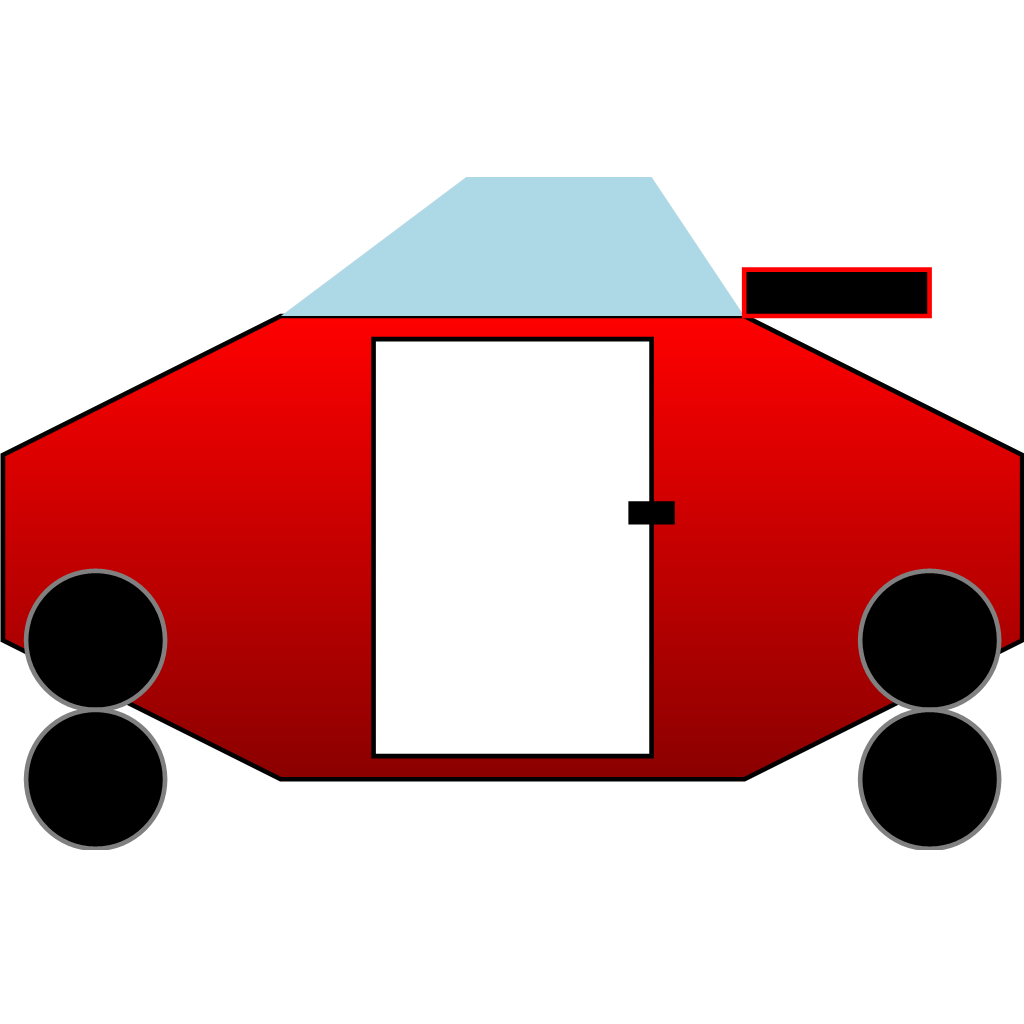
\includegraphics[width=0.16\textwidth]{Section 2/automobile_2d.png}
	\hspace{0.2in}
	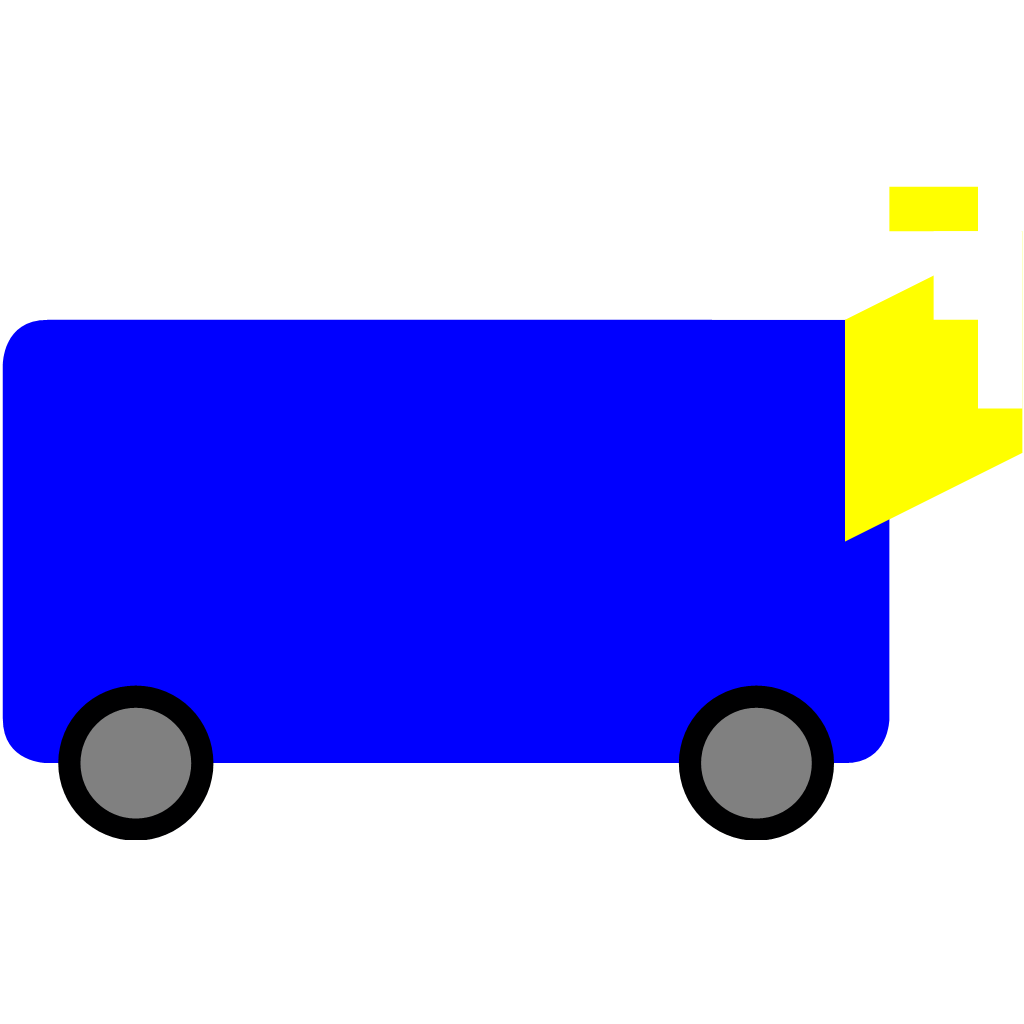
\includegraphics[width=0.16\textwidth]{Section 2/truck_2d.png}
	\hspace{0.2in}
	
\includegraphics[width=0.16\textwidth]{Section 2/cat_2d.png}
	\hspace{0.2in}
	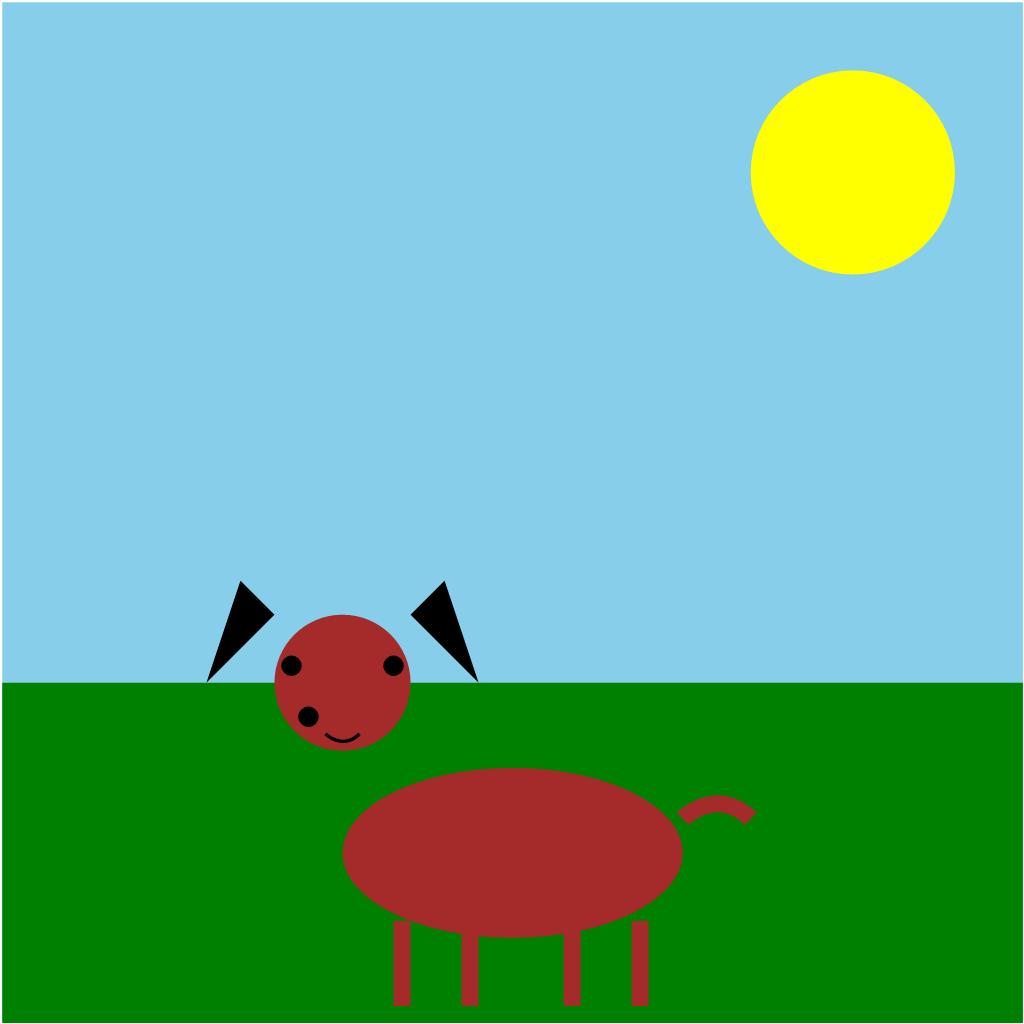
\includegraphics[width=0.16\textwidth]{Section 2/dog_2d.png}
	\caption{SVGs generated by \DV \ for the classes automobile, truck, cat, dog.}
	\label{fig:2d}
\end{figure}

\subsubsection{Image generation beyond memorization}
One may hypothesize, however, that the model simply copied the code from training data, where similar images appear. Given that the model was trained solely on textual content, one may further argue that there is no reason to expect that it would understand visual concepts, let alone that it would be able to create, parse and manipulate images. Yet, the model appears to have a genuine ability for visual tasks, rather than just copying code from similar examples in the training data. The evidence below strongly supports this claim, and demonstrates that the model can handle visual concepts, despite its text-only training.
\newline

In the first example we prompted the model to draw a person by combining the shapes of the letters Y, O and H (see Figure~\ref{fig:alphabetfigure} for the exact prompt and the result). 

\begin{figure}[h]
\begin{AIbox}{\DV}\vspace{-5px}
\parbox[t]{0.75\textwidth}{Produce TikZ code that draws a person composed from letters in the alphabet. The arms and torso can be the letter Y, the face can be the letter O (add some facial features)  and the legs can be the legs of the letter H. Feel free to add other features.}\hspace{50px}
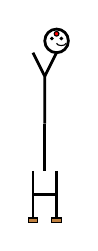
\begin{tikzpicture}[scale=0.3,baseline={(0,0.8)}]
	% Draw the Y
	\draw[line width=1pt] (0,0) -- (0,2) -- (-0.5,3); % left arm
	\draw[line width=1pt] (0,2) -- (0.5,3); % right arm
	\draw[line width=1pt] (0,0) -- (0,-2); % torso
	% Draw the O
	\draw[line width=1pt] (0.5,3.5) circle (0.5); % head
	\draw[fill=black] (0.3,3.6) circle (0.05); % left eye
	\draw[fill=black] (0.7,3.6) circle (0.05); % right eye
	\draw (0.5,3.4) arc (180:360:0.2 and 0.1); % mouth
	% Draw the H
	\draw[line width=1pt] (-0.5,-2) -- (-0.5,-4); % left leg
	\draw[line width=1pt] (0.5,-2) -- (0.5,-4); % right leg
	\draw[line width=1pt] (-0.5,-3) -- (0.5,-3); % crossbar
	% Add some features
	\draw[fill=red] (0.5,3.8) circle (0.1); % hat
	\draw[fill=brown] (-0.7,-4) rectangle (-0.3,-4.2); % left shoe
	\draw[fill=brown] (0.3,-4) rectangle (0.7,-4.2); % right shoe
\end{tikzpicture}

\tcbline
\parbox[t]{0.75\textwidth}{The torso is a bit too long, the arms are too short and it looks like the right arm is carrying the face instead of the face being right above the torso. Could you correct this please?}\hspace{50px}
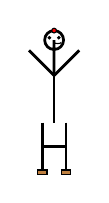
\begin{tikzpicture}[scale=0.3,baseline={(0,0.2)}]
	% Draw the Y
	\draw[line width=1pt] (0,0) -- (0,-2); % torso
	\draw[line width=1pt] (0,0) -- ++(135:1.5); % left arm
	\draw[line width=1pt] (0,0) -- ++(45:1.5); % right arm
	% Draw the O
	\draw[line width=1pt] (0,0) -- ++(90:1.5) circle (0.4); % head
	\draw[fill=black] (90:1.5) ++(-0.2,0.1) circle (0.05); % left eye
	\draw[fill=black] (90:1.5) ++(0.2,0.1) circle (0.05); % right eye
	\draw (90:1.5) ++(0,-0.1) arc (180:360:0.15 and 0.05); % mouth
	% Draw the H
	\draw[line width=1pt] (-0.5,-2) -- (-0.5,-4); % left leg
	\draw[line width=1pt] (0.5,-2) -- (0.5,-4); % right leg
	\draw[line width=1pt] (-0.5,-3) -- (0.5,-3); % crossbar
	% Add some features
	\draw[fill=red] (90:1.5) ++(0,0.4) circle (0.1); % hat
	\draw[fill=brown] (-0.7,-4) rectangle (-0.3,-4.2); % left shoe
	\draw[fill=brown] (0.3,-4) rectangle (0.7,-4.2); % right shoe
\end{tikzpicture}

\tcbline
\parbox[t]{0.75\textwidth}{Please add a shirt and pants.}\hspace{50px}
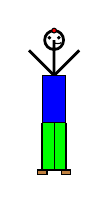
\begin{tikzpicture}[scale=0.3,baseline={(0,-0.4)}]
	% Draw the Y
	\draw[line width=1pt] (0,0) -- (0,-2); % torso
	\draw[line width=1pt] (0,0) -- ++(135:1.5); % left arm
	\draw[line width=1pt] (0,0) -- ++(45:1.5); % right arm
	% Draw the O
	\draw[line width=1pt] (0,0) -- ++(90:1.5) circle (0.4); % head
	\draw[fill=black] (90:1.5) ++(-0.2,0.1) circle (0.05); % left eye
	\draw[fill=black] (90:1.5) ++(0.2,0.1) circle (0.05); % right eye
	\draw (90:1.5) ++(0,-0.1) arc (180:360:0.15 and 0.05); % mouth
	% Draw the H
	\draw[line width=1pt] (-0.5,-2) -- (-0.5,-4); % left leg
	\draw[line width=1pt] (0.5,-2) -- (0.5,-4); % right leg
	\draw[line width=1pt] (-0.5,-3) -- (0.5,-3); % crossbar
	% Add some features
	\draw[fill=red] (90:1.5) ++(0,0.4) circle (0.1); % hat
	\draw[fill=brown] (-0.7,-4) rectangle (-0.3,-4.2); % left shoe
	\draw[fill=brown] (0.3,-4) rectangle (0.7,-4.2); % right shoe
	% Add a shirt and pants
	\draw[fill=blue] (-0.5,0) -- (-0.5,-2) -- (0.5,-2) -- (0.5,0) -- cycle; % shirt
	\draw[fill=green] (-0.5,-2) -- (-0.5,-4) -- (0,-4) -- (0,-2) -- cycle; % left pant
	\draw[fill=green] (0,-2) -- (0,-4) -- (0.5,-4) -- (0.5,-2) -- cycle; % right pant
\end{tikzpicture}

\end{AIbox}
	\caption{A stick figure composed of alphabet symbols}
	\label{fig:alphabetfigure}
\end{figure}

The letters of O, H and Y are created using draw-line and draw-circle commands and the model manages to position them in a way that results in a reasonably-looking stick figure. It is plausible that the training data contains information about the geometric shapes of different letters, and perhaps the fact that the letter Y could look like a torso with arms pointing upwards can also be inferred from the training data. Arguably, it is much less obvious that the model would be able to infer from the training data what is a reasonable way to position those letters in order to draw a reasonably-looking stick figure. In a second iteration, we prompted the model to correct the proportions of the torso and arms, and place the head in the center. Finally, we asked the model to add a shirt and pants (see Figure~\ref{fig:alphabetfigure} for the exact prompt and the result). To further probe the model's grasp of geometric concepts, we also asked it to create images that blend objects with letters of the alphabet. The model had to first invent a reasonable way of merging the object and the letter, and then produce the image. The results, shown in Figure~\ref{fig:alphabetfigure2}, demonstrate that \DV\ can usually preserve the identity of both the object and the letter and combine them in a creative way.

\begin{figure}
\begin{AIbox}{\DV}\scriptsize\vspace{-5px}
\parbox{1\textwidth}{\begin{alltt}
You will be given a name of an object (such as Car, Chair, Elephant) and a letter in the alphabet. Your goal is to first produce a 1-line description of how that object can be combined with the letter in an image (for example, for an elephant and the letter J, the trunk of the elephant can have a J shape, and for the letter A and a house, the house can have an A shape with the upper triangle of the A being the roof). Following the short description, please create SVG code to produce this (in the SVG use shapes like ellipses, triangles etc and polygons but try to defer from using quadratic curves).
\end{alltt}}
\vspace{-15px} \tcbline \vspace{-20px}
\parbox[t]{0.8\textwidth}{
\begin{alltt}
Round 1: A pig and the letter H. \\
\hl{Description: The pig can be lying on its back with its four legs forming the two vertical bars of the H, and its curly tail forming the horizontal bar.}
\end{alltt}
}
\makebox[0pt][l]{\raisebox{-55px}{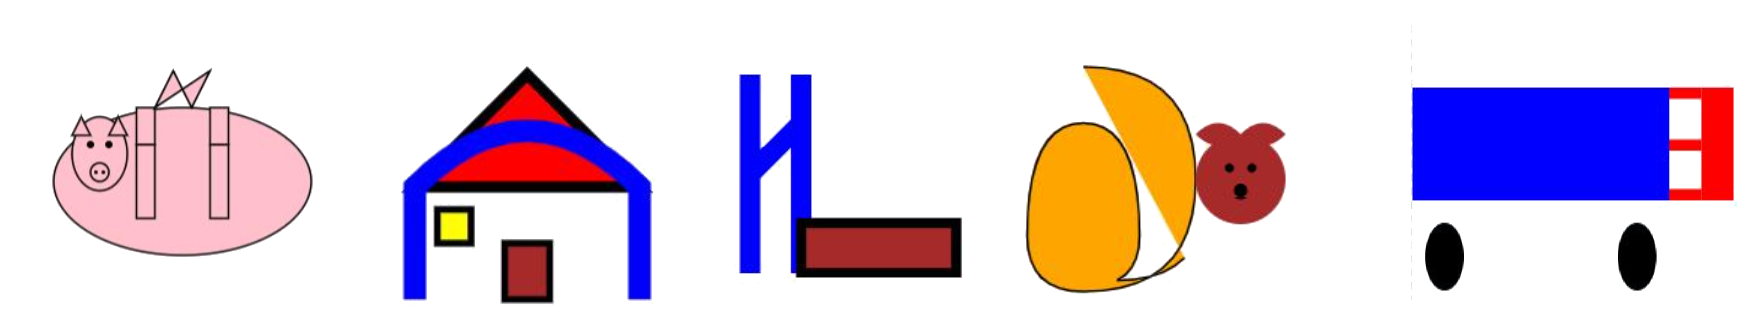
\includegraphics[trim={0 0 700 0},clip,width=0.2\textwidth]{Section 2/letters_objects.png}}}%
\vspace{-15px} \tcbline \vspace{-20px}
\parbox[t]{0.8\textwidth}{
\begin{alltt}
Round 2: A house and the letter U. \\
\hl{Description: A house with a U shape, where the two vertical lines of the U are the walls and the horizontal line is the floor. The roof is a triangle above the U.}
\end{alltt}
}
\makebox[0pt][l]{\raisebox{-55px}{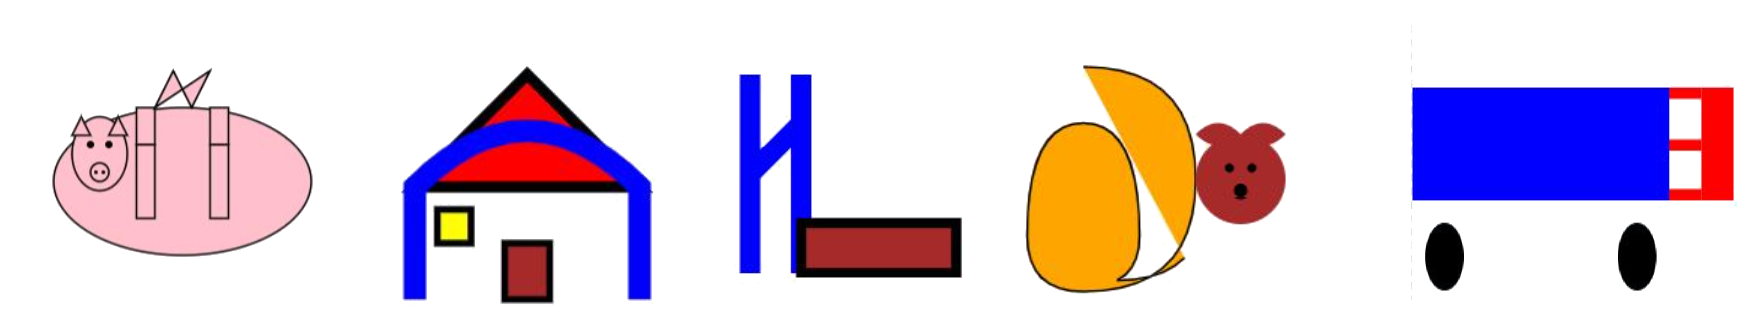
\includegraphics[trim={170 0 530 0},clip,width=0.2\textwidth]{Section 2/letters_objects.png}}}%
\vspace{-10px} \tcbline \vspace{-20px}
\parbox[t]{0.8\textwidth}{
\begin{alltt}
Round 3: A chair and the letter K. \\
\hl{Description: The back of the chair can have a K shape, with two vertical lines and a diagonal line connecting them. The seat of the chair can be a rectangle.}
\end{alltt}
}
\makebox[0pt][l]{\raisebox{-55px}{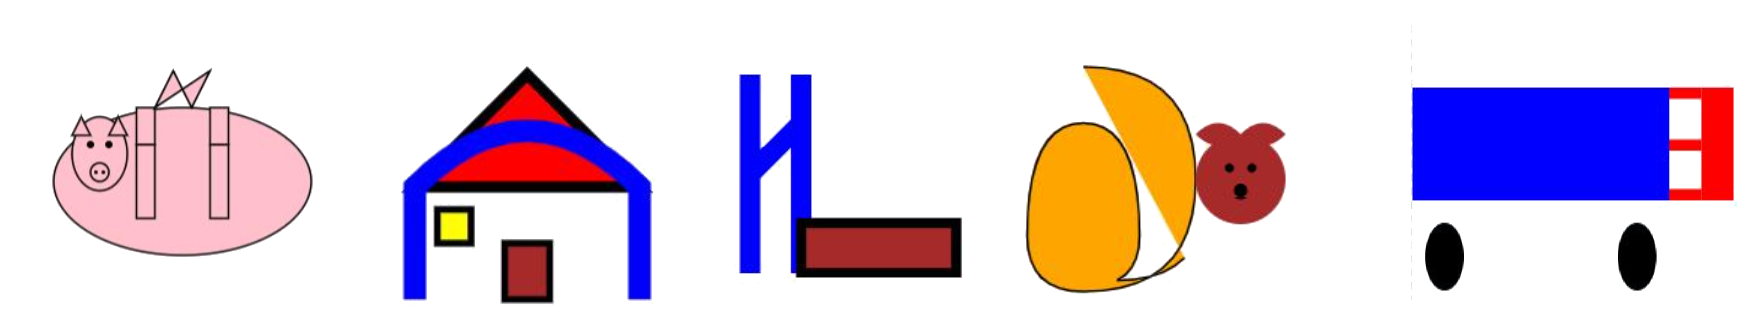
\includegraphics[trim={340 0 360 0},clip,width=0.2\textwidth]{Section 2/letters_objects.png}}}%
\vspace{-10px} \tcbline \vspace{-20px}
\parbox[t]{0.8\textwidth}{
\begin{alltt}
Round 4: A dog and the letter Q. \\
\hl{Description: The dog is sitting with its tail curled around its body, forming a Q shape. The Q is filled with orange and has a black outline.}
\end{alltt}
}
\makebox[0pt][l]{\raisebox{-55px}{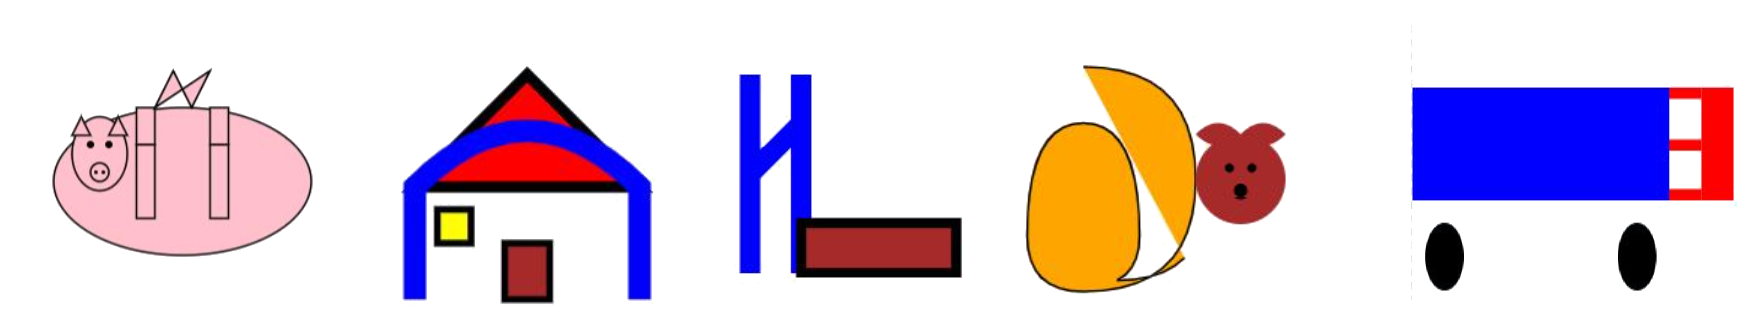
\includegraphics[trim={490 0 200 0},clip,width=0.2\textwidth]{Section 2/letters_objects.png}}}%
\vspace{-10px} \tcbline \vspace{-20px}
\parbox[t]{0.8\textwidth}{
\begin{alltt}
Round 5: A car and the letter E. \\
\hl{Description: The car has an E shape on its front bumper, with the horizontal lines of the E being lights and the vertical line being the license plate.}
\end{alltt}
}
\makebox[0pt][l]{\raisebox{-55px}{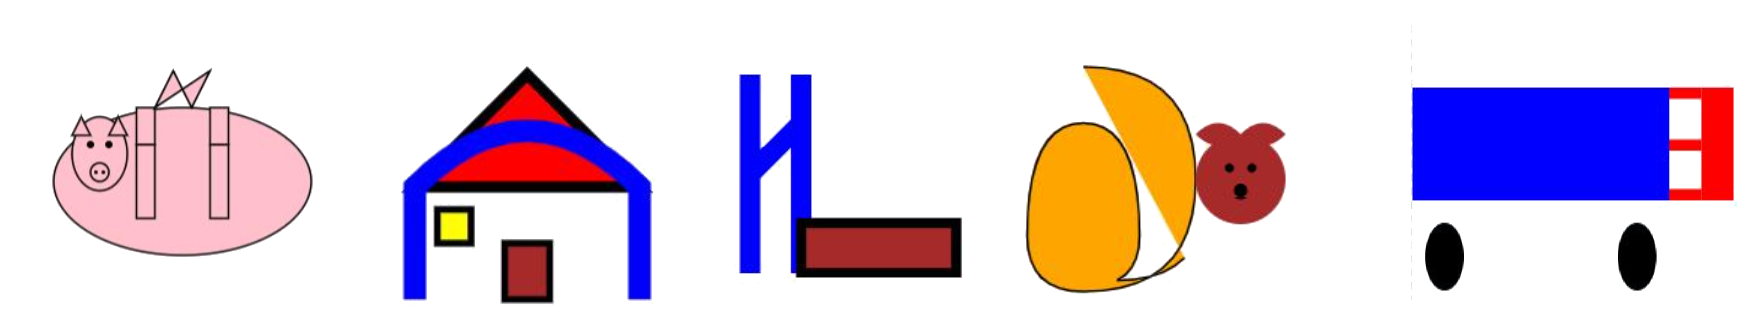
\includegraphics[trim={680 0 0 0},clip,width=0.2\textwidth]{Section 2/letters_objects.png}}}%
\vspace{-10px}
\end{AIbox}
	\caption{Images combining alphabet letters and objects.}
	\label{fig:alphabetfigure2}
\end{figure}

\subsubsection{Image generation following detailed instructions (\`a la Dall-E)}\label{sec:2d3d_example}
To further test \DV's ability to generate and manipulate images, we tested the extent to which it can follow detailed instructions on creating and editing figures. This task requires not only generative skills, but also interpretive, compositional, and spatial skills. 
\newline

The first example instructs the model to generate a 2D image with the description ``A frog hops into a bank and asks the teller, `Do you have any free lily pads?' The teller responds, `No, but we do offer low interest loans for pond upgrades.' ''. We made several attempts to generate the image, each time, the generation matches the description with the key objects frog, teller, bank, and the two texts. We picked the most visually appealing version. Inspired by the standard image generation workflow, we then ask \DV\ to upscale the figure by adding more details. \DV\ adds a bank sign, some windows, a car, a traffic light, a few clouds, and makes the frog hold a flower. Finally, we ask \DV\ to perform various tasks, such as adding a few objects relative to the existing objects, recoloring some objects and changing the z-order of some objects. \DV\ does all tasks correctly. The final result is shown in Figure~\ref{fig:multimodelinstr} (a) and the prompt in Figure~\ref{fig:2dprompt}.
\newline

Our second example is an attempt to generate a 3D model using Javascript. We instruct \DV\ with the prompt ``A fantasy landscape of floating islands, waterfalls, and bridges, with a dragon flying in the sky and a castle on the largest island." Similar to the 2D experiment, we ask \DV\ to modify the 3D model in various ways, such as adding, relocating, recoloring objects and changing the trajectory of the dragon. Again, \DV\ does many of the tasks correctly. The final result is shown in Figure~\ref{fig:multimodelinstr} (b) and the prompt in Figure~\ref{fig:3dprompt}. It is a 3D animation with multiple dragons is circling above the islands.

\begin{figure}[H]
	\centering
	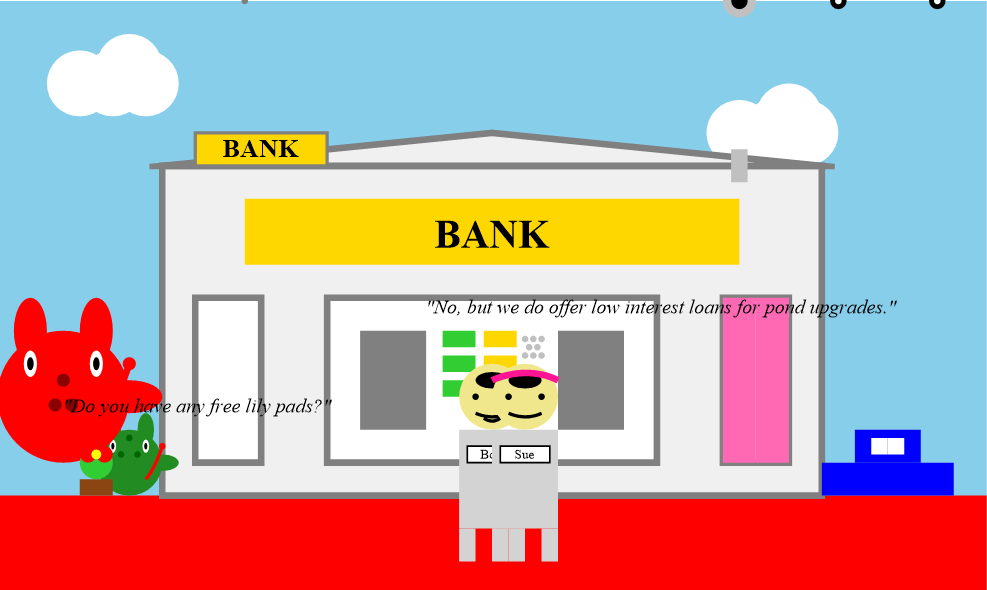
\includegraphics[height=0.3\textwidth]{Section 2/bank.png}
	\hspace{0.1in}
	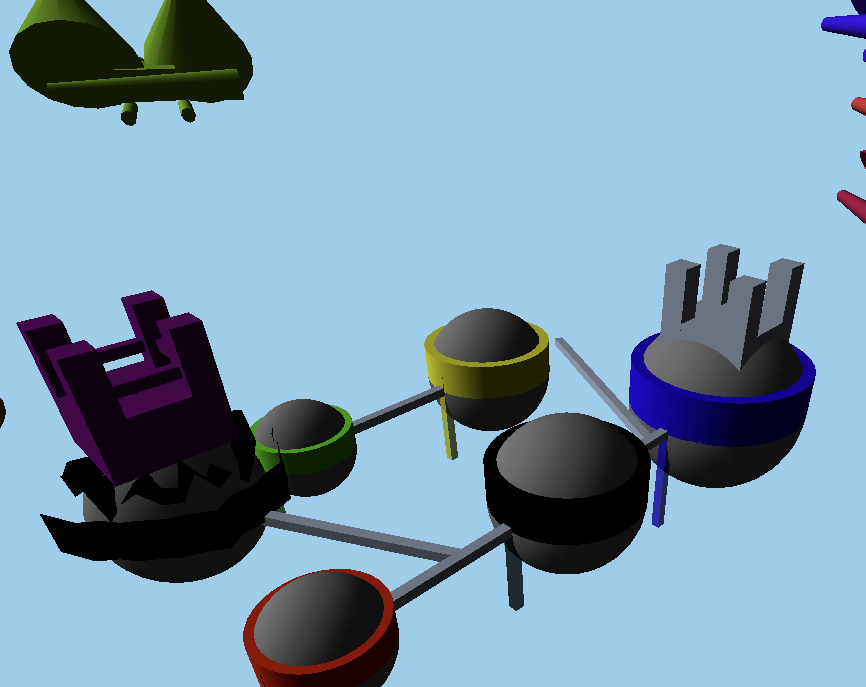
\includegraphics[height=0.3\textwidth]{Section 2/island.png}
	\caption{Examples of 2D, 3D images generated according to instructions.}
	\label{fig:multimodelinstr}
\end{figure}

\subsubsection{Possible application in sketch generation}
Text-to-image synthesis models have been widely explored in recent years, but they often suffer from a lack of spatial understanding capabilities and the inability to follow complex instructions~\cite{gokhale2022benchmarking}. For example, given a prompt such as ``draw a blue circle on the left and a red triangle on the right'', these models may produce images that are visually appealing but do not match the desired layout or colors. On the other hand, \DV\ can generate code from a prompt, which can be rendered as an image, in a way that is true to the instructions to a higher degree of accuracy. However, the quality of the rendered image is usually very low. Here, we explore the possibility of combining \DV\ and existing image synthesis models by using the \DV\ output as the sketch. As shown in Figure~\ref{fig:dv_stable}, this approach can produce images that have better quality and follow the instructions more closely than either model alone. We believe that this is a promising direction for leveraging the strengths of both \DV\ and existing image synthesis models. It can also be viewed as a first example of giving \DV\ access to {\em tools}, a topic we explore in much more depth in Section~\ref{sec:affordances}.

\begin{figure}[H]
\begin{AIbox}{\DV\ and Stable Diffusion}
{\bf Prompt:} A screenshot of a city-building game in 3D. The screenshot is showing a terrain where there is a river from left to right, there is a desert with a pyramid below the river, and a city with many highrises above the river. The bottom of the screen has 4 buttons with the color green, blue, brown, and red respectively. \\

\parbox{0.3\textwidth}{
{\bf \DV:}\\\ \\
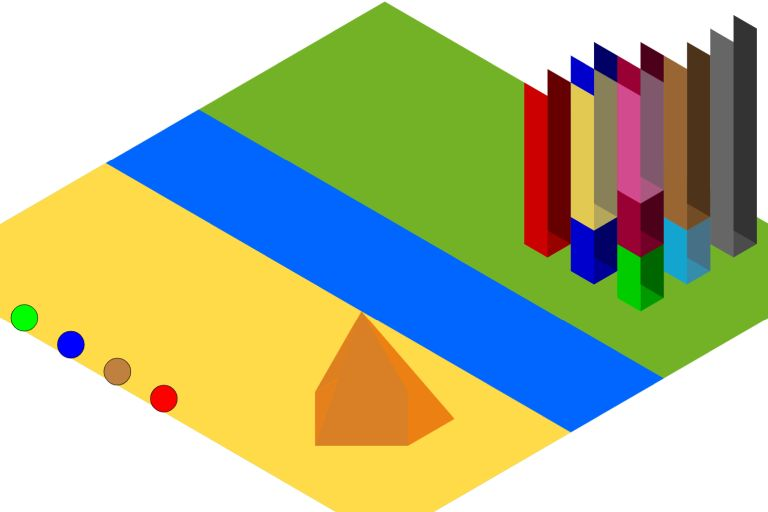
\includegraphics[width=0.3\textwidth]{Section 2/DV_city.png}
}
\hspace{10px}
\parbox{0.3\textwidth}{
{\bf Stable Diffusion v2.1:}\\\ \\
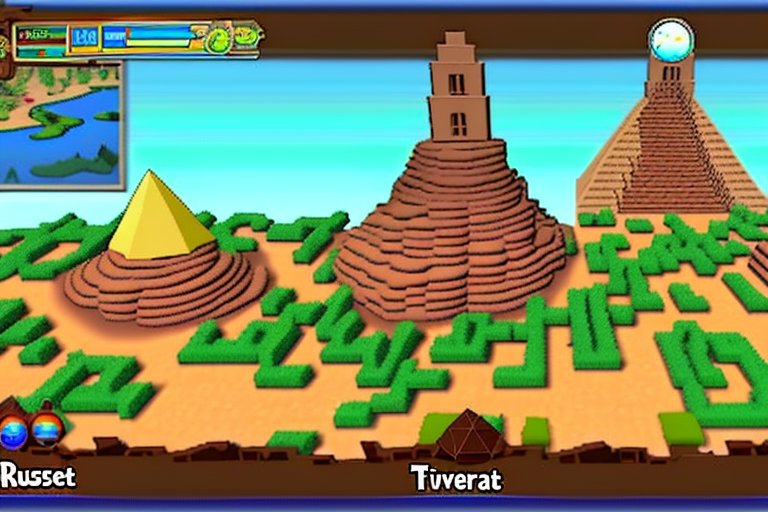
\includegraphics[width=0.3\textwidth]{Section 2/stable_city.png}
}
\hspace{10px}
\parbox{0.3\textwidth}{
{\bf Stable Diffusion v2.1 \\ with \DV's sketch:}\\
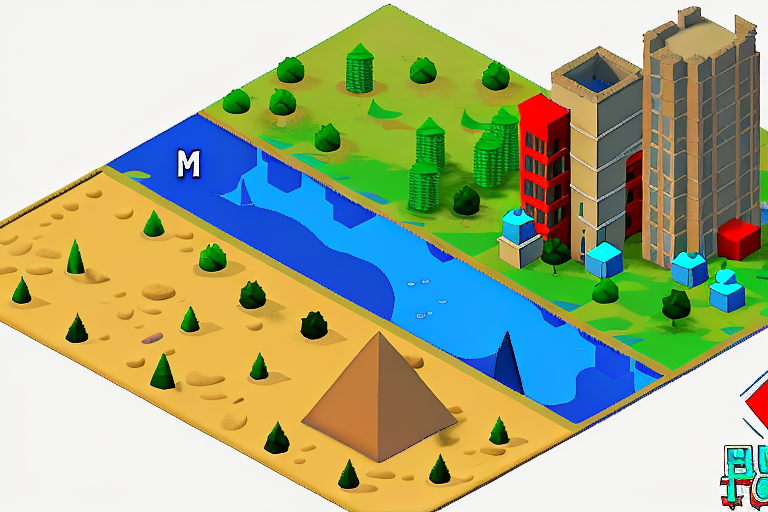
\includegraphics[width=0.3\textwidth]{Section 2/DV_stable_city.png}
}
\end{AIbox}
	\caption{Combining \DV\ and stable diffusion}
	\label{fig:dv_stable}
\end{figure}

\subsection{Music} \label{sec:music}
The data on which the model was trained also contains musical information encoded as ABC notation. This is a system that uses letters, numbers and symbols to represent musical pitches, durations, chords and other elements in a compact and readable way. We are interested in exploring how well the model has acquired musical skills from this exposure, such as composing new melodies, transforming existing ones, and understanding musical patterns and structures.

When instructed to generate a short tune (Figure~\ref{fig:music}), and the model was able to produce valid ABC notation. The tune had a clear structure, the time signature was consistent between bars and the notes followed increasing and decreasing patterns. The tune also used a consistent set of notes within the melody, and the rhythm had a repetitive pattern. However, the model did not seem to obtain the skill of understanding harmony. In fact, consecutive notes in the generated tunes are almost always adjacent to each other (namely, the note following C will almost typically be either B or D), and testing on 10 generated tunes, we were not able to extract any clear chords or arpeggios.

We then asked the model to describe the tune in musical terms. It was able to successfully give a technical description of the structure in terms of repetitions, the rising or descending parts of the melody and to some extent the rhythm. However, it seems that the descriptions of the harmony and chords are not consistent with the notes (in fact, it refers to sequences of adjacent notes, which do not form valid chords, as arpeggios).

We then asked the model to manipulate the melody in two ways. First, we instructed to change a certain rising sequence to a descending one, which it did successfully. Then we asked the model to convert the tune to a duet adding a bass voice. The model successfully extends the ABC notation with a second staff which has compatible rhythm and is played on a lower octave, however there is a lack of harmony between the two voices.

In summary, the model was able to produce valid tunes in ABC notation and, to some extent, explain and manipulate their structure. However, we could not get the model to produce any nontrivial form of harmony. It should be noted that ABC notation is not a very widely used format, and in fact the model was not able to produce even the most well-known tunes in ABC notation (such as Ode to Joy, F\"{u}r Elise or Greensleeves, all of which are abundant online in that format), nor was it able to recognize these tunes.
\begin{figure}[H]
\begin{AIbox}{\DV}\vspace{-5px}
\parbox{1\textwidth}{\scriptsize
\begin{alltt}
Can you compose a short tune (say four to eight bars) using ABC notation? \\
\hl{There are many possible ways to compose a short tune in abc notation, but here is one example:} \\

\hl{X:1\\
T:Example Tune\\
M:4/4\\
L:1/8\\
K:C\\
|:G2AB c2BA | G2AB c2c2 | edcB c2BA | G4-G2z2 :|\\
|:c2de f2ed | c2de f2f2 | g2fe d2cB | c4-c2z2 :|} \\

\hl{This tune has two four-bar phrases, each repeated once, forming an A part and a B part. The key is C major.} \\\vspace{-2px}

Can you describe the tune in musical terms?

\hl{Here is one possible description:

The tune starts with a rising arpeggio of the tonic chord (C major), followed by a descending scale that returns to the tonic. This pattern is repeated, but the second time the scale continues to the higher tonic note. The first phrase ends with a long tonic note.

The second phrase begins with a similar pattern, but using the subdominant chord (F major) instead of the tonic. The second time, the scale continues to the higher subdominant note. The phrase ends with a stepwise descent to the tonic, followed by a long tonic note.

The A part and the B part have a similar structure, but use different chords and ranges. The tune has a simple and catchy melody, with a clear sense of tonality and rhythm.}\\\vspace{-2px}

I like part A, but maybe part B is just a bit too similar to part A, making the song repetitive.  How about beginning part B with a descending arpeggio instead of a rising one?

\hl{Sure, that would create some contrast and variation. Here is one possible way to do that:

X:1\\
T:Example Tune\\
M:4/4\\
L:1/8\\
K:C\\
|:G2AB c2BA | G2AB c2c2 | edcB c2BA | G4-G2z2 :|\\
|:f2ed c2BA | f2ed c2c2 | g2fe d2cB | c4-c2z2 :|}\\\vspace{-2px}

That's much better. Now how about making this into a duet, can you add a second staff for this with a bass accompanying the melody?

\hl{One possible way to write a second staff for this tune is to use root notes and fifths of the chords, as well as some passing notes, to create a simple accompaniment. Here is an example in abc notation, with the second hand bass on the lower staff:

X:1 \\
T:Example Tune\\
M:4/4\\
L:1/8\\
K:C\\
V:1\\
|:G2AB c2BA | G2AB c2c2 | edcB c2BA | G4-G2z2 :|\\
|:f2ed c2BA | f2ed c2c2 | g2fe d2cB | c4-c2z2 :|\\
V:2 clef=bass\\
|:C,2C,2 G,2G,2 | C,2C,2 G,2G,2 | F,2F,2 E,2E,2 | C,4-C,2z2 :|\\
|:F,2F,2 C,2C,2 | F,2F,2 C,2C,2 | G,2G,2 F,2F,2 | E,2C,2 G,2C,2 :|}\\\vspace{-2px}

The sheet music of the final tune:
\end{alltt}\vspace{-10px}
\centering
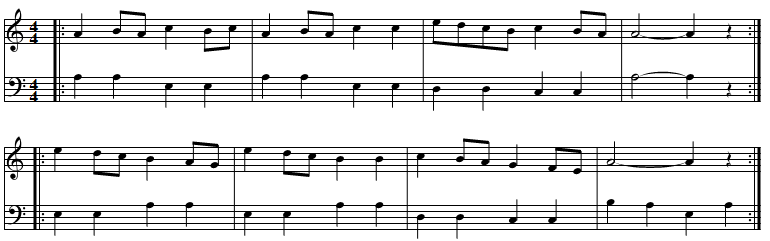
\includegraphics[width=0.9\textwidth]{Section 2/music.png}\vspace{-8px}
}
\end{AIbox}
\caption{Generating and modifying a tune in ABC notation.}
\label{fig:music}
\end{figure}